% Defined in the document class file (uqthesis.cls) are a number of options for the content of the formatted document.  These features are defined using the command (\DeclareOption).  We may control the expression of these options by adding the appropriate identifier to the list passed when calling the document class. This list is contained within square brackets. The following options exist:
%	honours				To change from default PHD structure.
%	printsupervisor			Print supervisors name on the title page.
%	printdepartment		Department name printed on title page.
%	printschool			School name printed on title page.
%	copyrightpage			Print copyright statement on back of title page.
%	examinerscopy			Print "Examiners Copy" bottom title page.
%	titlesmallcaps			Change the written font of the document title.
\documentclass [honours, printsupervisor, printschool, copyrightpage, titlesmallcaps] {uqthesis}

%%%%% Some helpful general definitions
\input{defs_thesis}

\begin{document}

\frontmatter

%%%%% Acknowledgements, titlepage, abstract, list of publications
% Logo located at top of title page.
\logo{figures/UQ_Logo.pdf}
\logoscale{1}

% Document & author titles.
\title{Correlated Errors on the Toric Code}
\author{Joshua M$^c$Donald}
\authorqual{Bachelor of Science with an Extended Major in Physics}
\supervisor{Associate Professor Thomas Stace and Dr Joshua Combes}
\department{ARC Centre of Excellence for Engineered Quantum System}
\school{School of Mathematics and Physics}

% Construct document with the following order. Comment out as necessary.
\titlepage

\chapter{Abstract}

The Toric code is a well known code for correcting errors on a quantum memory. Until now, all work with the Toric code has had the assumption that errors on the codespace are uncorrelated. The scheme used to correct these errors is optimized for uncorrelated error. In this thesis, I present an improved decoder for the syndrome of the Toric Code, that improves upon the success rate of the code, in recovering from correlated errors. This improvement should lead to helping realize quantum computing earlier, by making them more robust to realistic error models. 
\chapter{Acknowledgements}

I would like to thank Tom Stace, and Josh Combes primarily, for the patience, and understanding. They spent many hours helping me understand principals and guiding my work and investigation. \\
I would also like to thank my friends and family for their help and support during this time. 

\tableofcontents

\listoffigures
\listoftables
\chapter{List of Symbols}

% please change this list to suit your thesis

The following list is neither exhaustive nor exclusive, but may be helpful.
\begin{list}{}{%
\setlength{\labelwidth}{24mm}
\setlength{\leftmargin}{35mm}}
\item[$D(N)$] Pythagorean distance for a walk of N steps
\item[$M(N)$] Manhattan Distance for a walk of N steps
\end{list}



\mainmatter

%%%%% Introduction

\chapter{Introduction}


\section{Quantum Computing}
The computer age started in 1936 when A. M. Turing invented the first computer, which also bore his name. This computer led not only science, but arguably every aspect of life down an accelerated route to improvement due to the computational advantage that it gave. A new revolution began in 1980 through the work of Manin \cite{Manin1980}, when he described a new type of computing: Quantum Computing. 
\\\\ 
Different algorithms or problems can be attributed a level of complexity based on the time, or steps, it takes a machine to solve a problem in relation to the size of the problem. The main classes of interest are whether a problem scales exponentially with the problem size (inefficient to compute) or whether it scales polynominally with the problem size(efficient to compute).

The utility of quantum computing stems from a point made by Deutsch inn 1985 \cite{Deutsch1985}, that a problem need not have the same level of complexity when solved on different types of machines. This means that a problem which is difficult to solve on a Turing machine, may not be difficult to solve on another type of machine (such as a quantum computer). This point was confirmed in 1994 when Shor discovered the Fast Fourier Transformation Algorithm for quantum computers  \cite{Shor1994}; as the first example of an algorithm that is faster to solve on a quantum computer. This algorithm's use in compromising the security of public key encryption techniques greatly increased interest in quantum computing.
Since then, new algorithms with improved speed have been discovered for quantum computing. As these new algorithms are discovered, the utility of quantum computers increases. 
\\\\
The key component of a quantum computer is a new type of information, called the qubit. Qubits are physically realized by any two level quantum system. The state of a qubit can be described by the state $\ket{\alpha}$, in equation \ref{eq:qubit}.
\begin{align}
\ket{\psi} = \alpha\ket{0} + \beta\ket{1}\\
|\alpha|^2+|\beta|^2 = 1	
\label{eq:qubit}
\end{align}
Where $\alpha,\beta\in \textbf{C}$. For a qubit, the global phase is unobservable, while the local phase is observable. For this reason, we can make the simplification that $\alpha \in \textbf{R}, \beta \in \textbf{C}$.
\subsection*{Pure Vs. Mixed States}
The qubit takes a linear superposition of the base kets $\ket{0}$ and $\ket{1}$, to represent its state of $\ket{\psi}$. When the qubit is measured, its superposition will collapse onto one of the base kets, and an eigenvalue of one of the base kets will be measured with probabilities determined by $P(\alpha)=|\alpha|^2$ and $P(\beta)=|\beta|^2$. This is not to say that the qubit is ever actually in one of the states $\ket{0}$ or $\ket{1}$ before being measured (it is in fact in the state $\ket{\psi}$), but rather to say that the base kets are what state it is in \textbf{after} being measured, due to the measurement projecting onto the base kets. The base kets are simply a way to describe the state of the system. This describes the measurement of a \textit{pure state}. For a \textit{mixed state}, (which can be created through error processes) the measurement outcomes can appear similar, but they are two distinct cases. The uncertainty in measurement you get from a mixed state comes from uncertainty in the density matrix, whereas a pure state in a superposition has no uncertainty in it's density matrix; its uncertainty in measurement outcomes comes from the projective measurement made on the superposition. It is important to note that a mixed state is constituted of multiple pure states, and those states can be in a superposition of states; leading to 2 levels of uncertainty (one classical, and one quantum)
\\\\
For the base kets $\ket{0}$ and $\ket{1}$, there is a standard basis that is used. 
\[
\ket{0} = 
\begin{bmatrix}
1 \\
0 
\end{bmatrix},
\ket{1} = 
\begin{bmatrix}
0 \\
1 
\end{bmatrix}
\]
\\\\
As with any quantum system, it is difficult to isolate a quantum computer from its environment. This interaction causes the quantum state of the particles constituting the computer to decohere, introducing errors. 
The decoherance of the system is known as an error channel. Thus for a density matrix $\rho = \ket{\psi}\bra{\psi}$ we have;
$$\xi (\rho) = U\rho U^\dagger $$
where $U$ is some quantum operation. The general error channel is the Pauli channel shown in equation \ref{eq:pauli}\footnote{conjugates are hidden, as Pauli operators are Hermetian operators}.
\begin{equation}
\xi(\rho) = (1-P_X-P_Y-P_Z)\rho +P_XX\rho X+P_YY\rho Y +P_ZZ\rho Z
\label{eq:pauli}
\end{equation}
X, Y and Z refer to the Pauli matrices\footnote{see appendix \ref{app:pauli}}, and $P_X$, $P_Y$ and $P_Z$ refer to the probabilities of X, Y and Z errors occurring respectively.
\\\\
This Pauli channel says that any error on a qubit can be represented as a linear combination of no errors (I), Bit Flip Errors (X), Phase Errors (Z) and Bit Flip Phase Errors (Y). 

Thus, an error on a prepared state $\ket{\Psi}$ can be represented by:
\begin{align*}
\ket{\psi} \rightarrow (e_1I+e_2X+e_3Z+e_4Y)\ket{\Psi}
\end{align*}
For some error coefficients, $e_i$. For a general qubit $\ket{\Psi} = a\ket{0} + b \ket{1}$, the phase flip error corresponds to:
\begin{align*}
\ket{\psi} \rightarrow a\ket{0} - b \ket{1}
\end{align*}
And the bit flip error corresponds to:
\begin{align*}
\ket{\psi} \rightarrow b\ket{0} + a \ket{1}
\end{align*}
In contrast to a classical Turing computer, which only suffers from bit flip errors; the quantum computer has a new form of error to deal with, the phase error. This new error requires new methods, often adapted from classical error correction theory, to handle. 
\section{Error Correction}
Errors can be introduced during two key processes of quantum computing; innately in quantum memory, and dynamically during computation. Methods for the prevention or correction of these errors are given distinct titles to distinguish: `Quantum Error Correction (QEC)' for the recovery of errors in quantum memory, and `Fault Tolerance (FT)' to protect against the errors created during the encoding and decoding of information due to imperfect logic gates. 
\\\\
One way to implement  QEC is with error correcting codes (ECCs). For many such codes, protection against errors require a large overhead of `backup bits', whereby a logical bit is encoded into many physical bits. In a clasical system using bits, a majority vote of the values of these bits can be used to recover from errors. Generalizing this method to quantum computers encounters difficulty, as quantum computers utilize the qubit. 

%{\color{red} Here i will define what error correcting codes are, and some introductory stabilizer formalism.  stabilizers, generators, codespace, logical operators, hilbert space, commutation relation of stbilizers and codesapce, what are syndrome measurements, code words, generators, CSS codes? stabilizers form an abeilian group which preserve a degree of freedom -- > can all be measured simultaneously. what a stabilizer ECC is}


\subsection{Toric Code}
An important `building block' of many advanced QCCs that can handle both the bit and phase flip errors, is the Toric Code. The Toric Code, or rather Toric \textit{Codes} invented by Kitaev in 1997 \cite{1997} is a family of topological stabilizer codes. The Toric code has 2 degenerate ground states, which allow for 2 logical qubits to be encoded, onto $2L^2$ physical qubits.

This code applies to a $L \times L$ lattice with periodic boundary conditions, where qubits exist as sites on the grid. A grid with periodic boundary conditions is topologically equivalent to the surface of a torus. The Toric Code has the following important properties:
\begin{enumerate}
	\item Each measurement made involves at most 4 qubits
	\item The code can correct $\frac{L-1}{2}$ X and Z errors
\end{enumerate}
The measurements made on the toric code are known as \textit{Plaquette} and \textit{Star} operators, which are highlighted as the blue square and the red cross in figure \ref{fig:toricgrid} respectively. 

The check operators in the Toric code are formed from the tensor product of 4 Z operators operating on the 4 adjacent sites to the plaquettes. It is given by the operator;
\begin{equation}
Z_P = \otimes_{l\in P}Z_l
\label{plaquetteoperator} 
\end{equation}
Where $l\in P$ denotes the edges forming the plaquette's border.
The tensor product of the 4 X operators acting on the sites that meet (star operators in figure \ref{fig:toricgrid})) is given by; 
\begin{equation}
X_s = \otimes_{l\ni s}X_l
\label{staroperator} 
\end{equation}
Where $l\ni s$ denotes the edges meeting at the vertix.
The toric code is the space in which these operators act trivially. 
Topological codes like the Toric code are useful, as sites where the stabilizer measurements take the value -1 can be though of as locations with defects; as the check operators are spatially localized. When a site is subject to error, a pair of quasi particles known as anyons are created, which represent the end points of an error chain (E). 
\\\\
The Toric Code has $2L^2$ possible star and plaquette operators. However, the codespace is subject to two constraints:
$$\prod X_s = 1 $$
$$\prod Z_P = 1 $$
These constraints mean that not all of the stabilizers are independant, and thus we only need to measure $2L^2-1$ star and $2L^2-1$ plaquette operators.
\\\\
The stabilizers of the Toric code form an abelian group. This means that the stabilizers can be measured simultaneously. This is due to the stabilizers either having no shared site (trivially commuting) or exactly 2 shared sites. i.e;
$$[X_i,X_j] = [Z_i,Z_j] = [X_i,Z_j] = 0$$
For any $i$, $j$.
A logical Z operation on a the Toric Code corresponds to a string of Z operators in a homologically non-trivial cycle\footnote{see appendix \ref{app:cycles}} extending across the lattice. X operations are implemented in the same way. There are 2 symmetries for each types of operation (4 distinct operations) which operate on the 2 qubits. 

\begin{figure}
	
	\begin{minipage}[b]{0.45\textwidth}
		\centering
		\includegraphics[width = \textwidth]{figs/toricgrid.eps}
		\caption{A graphical view of the toric code. Qubits exist on/as edges of the lattice. A star operator is shown in red, and a plaquette operator is shown in blue.}
		\label{fig:toricgrid}
	\end{minipage}\hfill
	\begin{minipage}[b]{0.45\textwidth}
		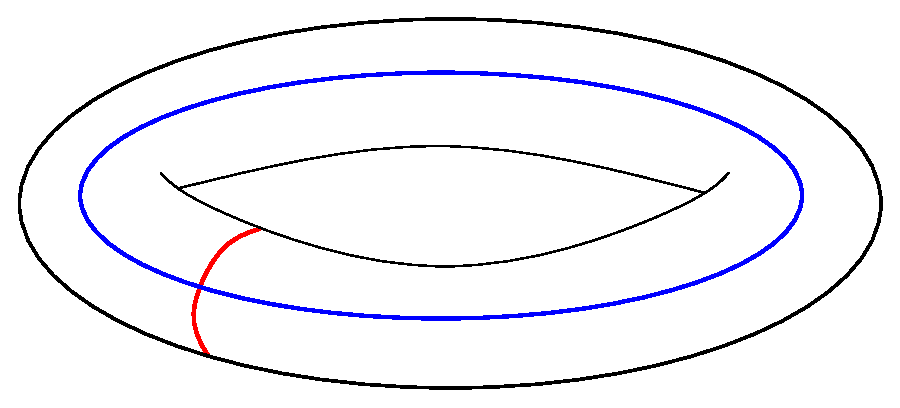
\includegraphics[width = \textwidth ]{figs/torus.eps}
		\caption{A torus has 2 possible non-contractible loops highlighted in red and blue. These loops can be formed from either X or Z Pauli operators.}
	\end{minipage}
	\caption{}
	
\end{figure}
An interesting characteristic of the toric code is that due to the dual-lattice nature, X and Z errors can be dealt with the same way, through the use of a Hadamard gate\footnote{See appendix \ref{app:hadamard}}. For conciseness, simulations were only performed with X errors. 
\\\\
The easy scalability of the toric code, and its position as the simplest topological code, make it both a central idea, and an important subject of study in regards to quantum error correction.
\\\\
In regards to figure \ref{fig:toricgrid}, an odd number of blue loops or an odd number of red loops, constitutes a logical error. This error is due to the loops forming homologically non-trivial topologies. If an even number of red, or an even number of blues loops are formed, then the topology that is formed is homologically trivial, and has no effect on encoded qubits. If a red and a blue loop form, then the resulting topology is also trivial, with no effect on the logical qubits. These trivial topologies mean that the topology of the surface (state of the qubit) is left unchanged. 
\\\\
To determine if the correction procedure was a success, the cycles $D = E+E'$ can be evaluated to check if the homology has changed. If the homology class of the cycle $D$ is non-trivial, then the code is no longer in the ground state, and encoded information has be changed\footnote{see appendix \ref{app:cycles} for more information on trivial/nontrivial cycles}. Errors form 1D chains taking the system out of its ground state, and into an orthogonal subspace. Correction procedures attempt to fix this by connecting chains into complete cycles. If the cycles that the correction procedure are homologically trivial, then the codespace gets mapped to itself in a non-trivial way, and the encoded information is lost. If the cycles are trivial however, then the information is protected.

Errors on the toric code are enacted through chains of Pauli operators, denoted as $E$. These chains preserve the code space if the chains of errors form cycles on the lattice. That is to say that the sites acted upon by Z operators must form cycles on the lattice, and sites acted upon by X's must form cycles on the dual lattice. 

Decoding the syndrome of the Toric Code consists of matching anyons (measurable end points of the error chains) together to create homologically trivial cycles. The correction path is denoted $E^\prime$.


\section{Random-Bond Ising model}
	Decoding the syndrome of the Toric Code for an uncorrelated error model was show by Dennis et al \cite{Dennis2001}, to be the same as solving the random-bond Ising model (RBIM) in 2D. The result of this work showed that optimal matching procedure for this error model is a least weight matching between syndrome measurements of -1. In this model, degenerate least weight paths have no effect. Recent studies by Stace and Barret \cite{Stace2010} and Dennis et al\cite{Dennis2001} have shown that the degeneracy of the matching path has an appreciable effect on the success rate of the code. The model implemented in this project however, ignores the effect of degeneracy, and chooses a random path from the degenerate matchings. This decoding step is shown in figure \ref{fig:graphicaloutput}, with a red error chain ($E$) and a yellow least weight path matching ($E^\prime$) the green anyons (Ising vorticies).
	
	\begin{figure}[htpb]
	\centering
	\includegraphics[width=0.5\textwidth ]{figs/graphicaloutput.png}
	\caption{A 5 by 5 torus. Blue dots indicate aligned regions ($\tau = +1$), red dots indicate unaligned ($\tau = -1$). The red lines show the one dimensional chains of antiferromagnetic bonds ($E$), which terminate in Ising vorticies (green dots). These Ising vorticies are then least weight matched ($E'$, in yellow).}
	\label{fig:graphicaloutput}
	\end{figure}
	
	This model is analogous to our treatment of a qubit prone to a single type of error. Spins in this model anti-align with probability $p$ and align with probability $1-p$. Spins that are align have the value $\tau_{ij}=+1$ and spins that anti-align take the value $\tau_{ij}=-1$. Again, if an odd number of spins in a plaquette have $\tau_{ij}= -1$, then that plaquette is the location of an Ising vortex, and analogously for star stabilizers.
	
	Applying the RBIM model can give new insights in possible ansatz with which to make predictions about how the code behaves. 

\section{Scaling}
	When using a least weight matching procedure derived from the RBIM model, the Toric code a has a critical error rate $p_{c0}$, below which large loops (more likely to be topologically nontrivial) are suppressed, and above which larger loops are promoted. This provides the toric code with a high chance of success below the threshold $p_{c0}$, and a low chance of success above the threshold. As $L\rightarrow \inf$ ; the transition between suppression and promotion of large loops leads to a discontinuity in $P_{success} \propto p$, where $P_{success}$ is the rate at which the encoded information is protected. This behaviour as the code scales with L can be described by the critical exponent $v_0$, and the critical point $p_c0$. The critical exponent characterizes that rate at which the average chain length (correlation length of the 1D chains) diverges from L. The relation between these values is shown in equation \ref{eq:scalingrelation}.
	
	\begin{equation}
	 x = (p-p_{c0})L^{1/v_0} 
	 \label{eq:scalingrelation}
	\end{equation}

	This relation allows us to map from 3 variables ($L$, $p$, $P_{success}$), into 2 ($x$, $P_{success}$), and lets us compare data between different code sizes (for sufficiently large L). The critical exponent and the critical point can be found experimentally. The critical point can be found by determining at what point lines of $P_{success} \propto p$ cross. The critical exponent can be found through variation, and optimizing for when the curves of $P_{success} \propto p$ are parallel. 

	The $E$ and $E^\prime$ are dependant upon L being even or odd. For this reason, we will find unique $v_0$ and $p_{c0}$ for the even and odd cases.
\section{Random Walks}
	\subsection{Random walks}
	Random walks can take several forms. 
	\begin{itemize}
		\item self avoiding random walk
		\item non-self avoiding 
		\item other variation $\cdots$ self flipping? non inverting or whatever.. have written in logbook...
	\end{itemize}
 	non-self avoiding random walks are the kind of error that this thesis investigates. 
 	This kind of random walk on a 2D grid has 4 possible moves at every timestep, and can move a distance of 1. 
 	These random walks can be characterized by their expected walk length. The expected walk length can take several forms.
 	By far the easiest to calculate walk length is the root-mean-square (RMS) walk length. This walk length is simply proportional to RMS of the number of steps. 
 	\begin{equation}
 	RMS(N) = \sqrt{N}s
 	 \end{equation}
 	The second type of distance, is the average Pythagorean distance. This distance is more complicated to calculate, and is found through the equation \ref({eq:pythag}
 	
 	Expected Pythagorean distance:
 	\begin{equation}
 	D(N) = \frac{1}{4^N}\sum_{i=0}^{N}\sum_{j=0}^{N}\prescript{N}{}{C}_{i}\prescript{N}{}{C}_{j} \frac{1}{\sqrt{2}}\sqrt{(2i-N)^2+(2j-N)^2)} 
 	\end{equation}
 	
 	Expected Manhattan distance:
 	\begin{equation*}
 	D(N) = \frac{1}{4^N}\sum_{i=0}^{N}\sum_{j=0}^{N}\prescript{N}{}{C}_{i}\prescript{N}{}{C}_{j} \frac{1}{\sqrt{2}} 
 	\begin{bmatrix}
 	1&1\\
 	\end{bmatrix} 
 	\left|
 	\begin{bmatrix}
 	\frac{1}{\sqrt{2}} & \frac{1}{\sqrt{2}} \\
 	\frac{-1}{\sqrt{2}} & \frac{1}{\sqrt{2}} 
 	\end{bmatrix}
 	\begin{bmatrix}
 	2i-N \\
 	2j-N
 	\end{bmatrix}
 	\right|
 	\end{equation*}
 	
	These formulas line up well with plots made from the distributions of simulated walks. 
	Figure \ref{fig:dists} shows how these mean values compare to the shape of the distributions. Figure \ref{fig:dists} shows gamma functions fitted to data of the manhattan distance and the pythagorean distances of the end points of 10,000 random walks. 
	
	\begin{figure}
		\centering
		\includegraphics[width = 0.8\textwidth]{figs/randomwalkdistribution_1000000_32}
		\label{fig:randomwalkdistributions}
		\caption{This figure is a PDF of the distance of generated random walks, with the distance calulated in different ways}
	\end{figure}
	important walklengths in figure \ref{fig:randomwalkdistributions} are the three calculated mean distances, and the locations of the turning points for the gamma distributions. 
	\begin{table}
	\centering
	\begin{tabular}{c c}
	Manhatten expected&  6.358192239869876\\ 
	Pythagorean expected&  5.016712342283284\\ 
	$\sqrt{N}$ &  5.6568542494923806\\ 
	Pythagoren PDF TP &  4.2506712139429359\\ 
	Manhattan PDF TP &  5.1970956125713439\\ 
	\end{tabular} 
	\caption{Important points from the PDFs for a walk length of N=32. }
	\label{tab:candidates}
	\end{table}
	The points in table \ref{tab:candidates} are potential candidate parameters for correction functions for correlated error models. 

 	The probability density function (PDF) in figure \ref{fig:randomwalkdistributions} were generate using Markov Chain Monte Carlo (MCMC) methods. These PDFs were then used to create a more accurate correction function for the Toric Code, as when we know that the distribution looks like figure \ref{fig:randomwalkdistributions} rather than an exponential decay (as in the non-correlated model), we can conclude that correcting proportionally to this distribution, rather than as simply a linear scale with distance; we should see an improved success rate of the code. 
 
 \subsection{Random walks again}
The distribution of random walks was shown by Lord Rayleigh \cite{bibid} to be approximated by the Rayleigh equation for diffusion for large step sizes. Computationally, large step sizes are very hard to compute for large samples of random walks. Here we develop exact solutions for random walks, to determine the expected walk length of a random walk after $N$ steps. We determine the expected walk length in terms of the Manhattan distance, and the Pythagorean distance, as both are of importance to the match scheme for correlated errors on the Toric code. We shall then confirm the results of these equations to the PDFs of simulated random walks, and the Rayleigh equation for diffusion. 

Firstly, the Rayleigh equation for diffusion:
\begin{equation}
P_N(R) \sim \frac{2R}{N}e ^{-R^2/N}
\label{eq:rayleigh}
\end{equation}
In 1906 Rayleigh proposed a method to calculate the PDF of a random walk for large N \cite{Rayleigh1905}. Here we show an exact method for determining the expected walk length; which is useful for our purposes of creating a correction function based upon a gaussian centred at that distance.  

\begin{align}
P_N(L) & = \frac{\sum_{i\in \mathds{S}}\sum_{j\in \mathds{S}} {}^NC_i {}^NC_j - \sum_{i\in \mathds{P}}\sum_{j\in \mathds{P}} {}^NC_i {}^NC_j}
{\sum_{i = 0}^N\sum_{j=0}^N {}^NC_i {}^NC_j }\\
\label{eq:exactPDF}
\end{align}
Where 
\begin{align}
\centering
	\mathds{S} &= \{ \frac{N-L}{2} \leq n \leq \frac{N+L}{2};  \hspace{1cm} n\in \mathds{Z}^{even} \}\\
	\mathds{P} &= \{\frac{N-L}{2}+1 \leq n \leq \frac{N+L}{2}-1;  \hspace{1cm} n\in \mathds{Z}^{even}\}
\end{align}
Where we define the sum of a null set to be zero. 


\begin{figure}
\centering
\includegraphics[width = 0.7\textwidth]{figs/calculatedvssimulated.pdf}
\caption{A comparison of the calulated values vs simulated walk data for 1,000,000 random walks. RMS error between the two trends was 7e-06. }
\label{fig:exactproof}
\end{figure}
Figure \ref{fig:exactproof} shows excellent agreement of formula \ref{eq:exactPDF} to walk data. 



\begin{figure}
\centering
\includegraphics[width = 0.7\textwidth]{figs/exactPDF.pdf}
\caption{This figure shows the exact PDF calculated for walks of various lengths. This data is generated from equation \ref{eq:exactPDF}.}
\end{figure}







\section{Correlated Errors}
	The recovery process (pairwise matching) is shown to be most effective when it is least weight \cite{Dennis2001}. Least weight matching is however only true for uncorrelated errors.
	Correlated errors can arise when nearby qubits are not well isolated from one anther, and this can allow errors to `walk' from qubit to qubit.

 	\subsection{Correlated errors}

	In the case of correlated errors, matchings that are similar in length to the average length of a random walk are more preferential for successful matchings. This length of walk can be used to improve the recovery process. The correlation length that the recovery process optimizes for can either be fixed, or can be adaptive as an ancilla memory gains information about the system. Information from the syndrome can be used to determine the correlation length and improve the code over time. 
	\\\\
	The schematic (figure \ref{fig:schematic}) shows how this toric code can then be used to feedback information over many cycles to store knowledge about the errors and to improve its correction rate over time. Information about error gained from the syndrome measurements can be stored in ancilla qubits, for use in `training' the decoder to optimally decode correlated errors.
	
	\begin{figure}[htpb]
	\centering
	\includegraphics[width =0.8\textwidth]{figs/schematic.eps}
	\caption{The logical qubits are encoded into the Toric code as $2$ logical qubits onto $2L^2$ physical qubits. These qubits then pass through an error channel. The syndrome is then measured, and an appropriate correction procedure takes place. The code is then decoded, and checked for success. }
	\label{fig:schematic}
	\end{figure}




%%%%% Other chapters in here

\chapter{Methods}
\section{Toric Code and Syndrome Measurements}
\subsection{Qubit layout and operators}
	The Toric code exists on a L by L lattice, consisting of $2L^2$ physical qubits. Ths lattice has periodic boundary conditions. For every row of the lattice there are 2 qubits at every site; forming a grid and a cogrid. The arrangements of the grid allows for plaquette operators to exist at every (i,j) site on the grid. Every plaquette operator is bordered by 4 qubits.
	
	Each qubit on the grid can take the value of -1 or 1, and its value is stored in a L by 2 by L array ($Q(L,2,L)$), to store the information about the grid and cogrid qubits. 
	
	Plaquette operators are stored in a L by L array ($S(L,L)$), and can also take the value of -1 or 1. 
	
	All qubits on the torus are initialized to to an error free state represented by `1'. When a physical qubit on the torus experiences an error, it's value is changed to `-1'. 
	
	 The syndrome of the code is determined through measuring all of the plaquette operators. A measurement of a plaquette opertor corresponds to;
	 \begin{equation}
		P_{i,j}=Z_{left} \otimes Z_{right} \otimes Z_{above} \otimes Z_{below} 
		\label{eq:plaquette]}
	 \end{equation}
	Equation \ref{eq:plaquette]} states that the value of plaquette i is equal to the measurement a Z operator on each neighbouring qubit. This corresponds to each value $P_i$ in the L by L plaquette array equalling the multiplication of the values of the surrounding qubits. i.e. multiply together the values of the qubits located at left, right, above and below the stabilizer. 
	\begin{equation}
		S(i,j) = 	Q(i,0,j)\cross Q(i,1,j)\cross Q(i+1,0,j+1) \cross Q(i+1,1,j+1)
	\end{equation}
	
	The measurements of the stabilizers creates an array called the syndrome, which consists of the locations of all the anyon locations,represented by -1's. 
	
	The syndrome measurement reveals information about the error locations on the torus. 
	A successful correction operation on the toric code must return the codespace to its ground state. The ground state of the toric code is degenerate, and is formed from the stabilizer space of the code. That is, any state which can be formed from a product of stabilzers, is a ground state of the code. The ground state of the toric code is populated by homologically trivial loops of -1's on the grid. A correction scheme on the toric code would aim to match any errant pairs of -1's in the stabilizer array (which indicate the end points of error chains), in an attempt to forms error-loops which are trivial, and return the code to its ground state.
	
	After applying these flips, the homology class of the code is determined by measuring a two test line of operators across the code in conjugate directions. If the eigenvalue of one of these measurements is -1, then there exists a nontrivial cycle, and the qubit representing that direction failed to be recovered from error. 
	\section{Uncorrelated Errors}
	Two error models were implemented. Firstly, an uncorrelated error model was used to validate the function of the code. The results from this uncorrelated error model was compared to \cite{Stace2010} for confirmation. 

	The uncorrelated error model was implemented by looping over every element in the qubit array, and flipping a qubits state with probability $p$. 
	The optimal decoding solution for this error model is to match anyons with least weight. A matrix of distances between anyons can be generated and passed to an implementation of Edmonds perfect matching. Kolmogorov's BlossomV code \cite{Kolmogorov2009} is a suitable implementation of this least-weight perfect-matching algorithm. This uncorrelated error model is analogous to noise on the qubits.

	\section{Correlated Errors}
	Random walks were used to simulated correlated errors on the toric code. 
	A random point on $Q$ was chosen as the starting point for the random walk. From this position, errors were designed to walk diagonally around the grid. Due to the offset nature of Q, diagonal movements are the shortest distance movements that anyons can make around the grid, and are therefore most likely. The walker was allowed to evolve for $N$ steps (the correlation length), with each movement direction being equally likely. 
	All locations that the walker moved to were then flipped.
	
	\section{Improved Decoders}
	Two new decoders are proposed to reduce the failure rate of correlated errors. Random walks have been shown to have expected Manhattan walk lengths \ref{eq:manahat_expected}. We postulate increasing the chance of matchings near this expected length should decrease the failure rate of the code. 
	
	We will heuristically investigate the effect of concatenating the least weight perfect matching procedure of the naive decoder with a reduction in weight around various distances.
	
	The improved decoders present make use of the same BlossomV matching algorithm of the least weight decoder. The new decoder add preference to selecting matches at new locations, but reducing the `perceived distance' that the blossomV code passes. Thus, to increase the weight of a pair for matching, the adjusted distance is reduced from the original Manhattan distance. 
	\subsection{Gaussian Decoder}
	
	The first method of optimizing for correlated errors, is to use a gaussian correction to offset the effect of correlating the errors. The optimal gaussian to reduce the failure rate of the code can be found by varying the parameters of the gaussian. To do so, the center of the gaussian is swept through [0,N] and the variance of the gaussian is swept though(0,$\sigma_{max}$]. The strength of the gaussian correction is held constant to reduce the computational overhead. The naive decoder has been proven to yield the lowest error rates when error is uncorrelated. For uncorrelated errors, the most common chain length is 0. A heuristic argument can be made that if the walk is not most likely to be at 0 (as is the case for correlated errors \ref{fig:exactpdfs}), then there is no reason to preference this length of walk over other lengths (for example, the expected walk length). 
	\\\\
	The gaussian correction reduces the Manhattan distance of anyons near the centre of the gaussian ($\overline{w}$).  It does so by creating a gaussain centred at $\overline{w}$, with variance $\sigma^2$; and then inverting it, and shifting it up by unity. 
	\begin{align}
	A &= M \left( 1 - e^{\frac{-(M-\overline{w})^2}{2\cdot \sigma^2}} \right) 
	\label{eq:gaussainadjust}
	\end{align}
	Equation \ref{eq:gaussainadjust} shows how the adjustment works. In equation \ref{eq:gaussainadjust} $A$ represents the adjusted value, $M$ is the original Manhattan distance, $\overline{w}$ is the centre of the gaussain, and $\sigma^2$ is the variance or width of the gaussain.
	The behaviour of this decoder is shown in figure \ref{fig:gaussiancorrection}. The expected walk length of a N=32 walk is 5.016; figure \ref{fig:gaussiancorrection} is typical of a gaussian that is closely `centred' at this expected walk length.
	\begin{figure}
		\centering
		\includegraphics[width = 0.7\textwidth]{figs/gaussian-20.png}
		\caption{The behaviour of the Gaussian decoder. The decoder reduces the adjusted distance near a chosen Manhattan distance.}
		\label{fig:gaussiancorrection}
	\end{figure}
	\subsection{Manhattan PDF Decoder}
	
\chapter{Results}
	A model has been implemented which simulates 3 types of errors. The code has also been adapted to run on a computing cluster with multi-threading. This performance boost to the code allows for very large code sizes to be investigated, with multiple variables. Corroboration of results with literature has also been performed. Figure \ref{fig:unscaled} and figure \ref{fig:scaled} show how after the scaling factor in equation \ref{eq:scalingrelation} has been applied with $v_c = 1.49$ and $p_c = 0.103$, the various code sizes come into close agreement. These values agree with those determined by Stace and Barret \cite{Stace2010}, and Deutch et al \cite{Deutsch1985}.
	\\\\
	\begin{figure}[htpb]
	\begin{minipage}[t]{0.48\textwidth}
		\centering
		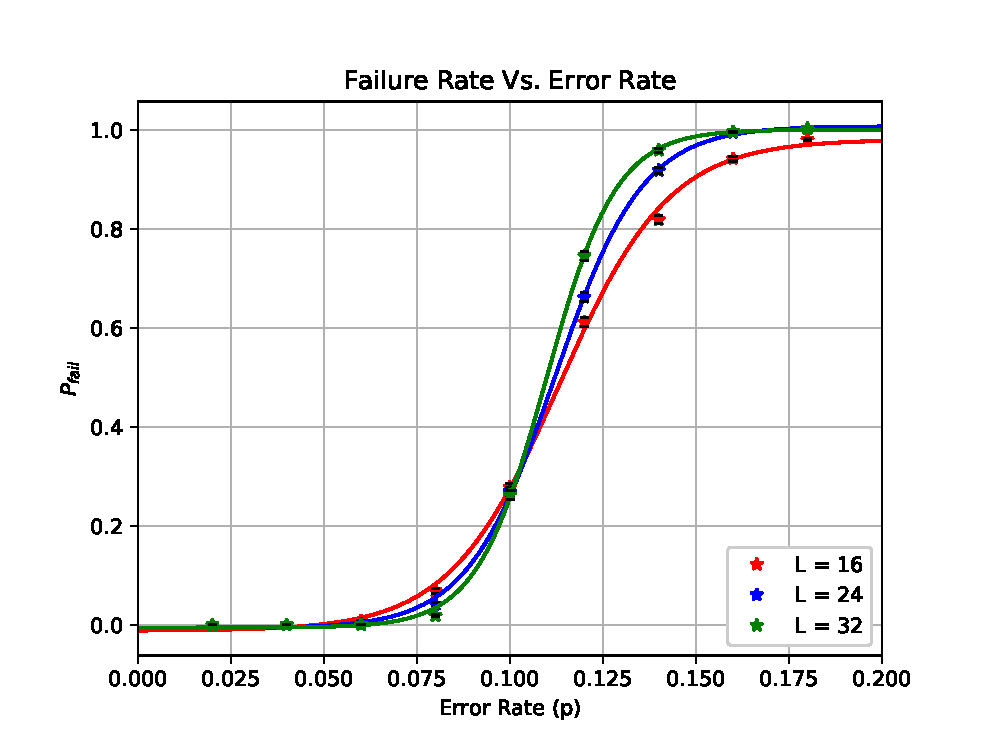
\includegraphics[width = \textwidth]{figs/unscaled.eps}
		\caption{This plot shows $P_{fail}$ Vs $p$ without any scaling applied, for 3 code sizes. A hyperbolic tangent trendline was fitted to allow the crossover point to be determined. Error bars have been plotted.}
		\label{fig:unscaled}
	\end{minipage}\hfill
	\begin{minipage}[t]{0.48\textwidth}
		\centering
			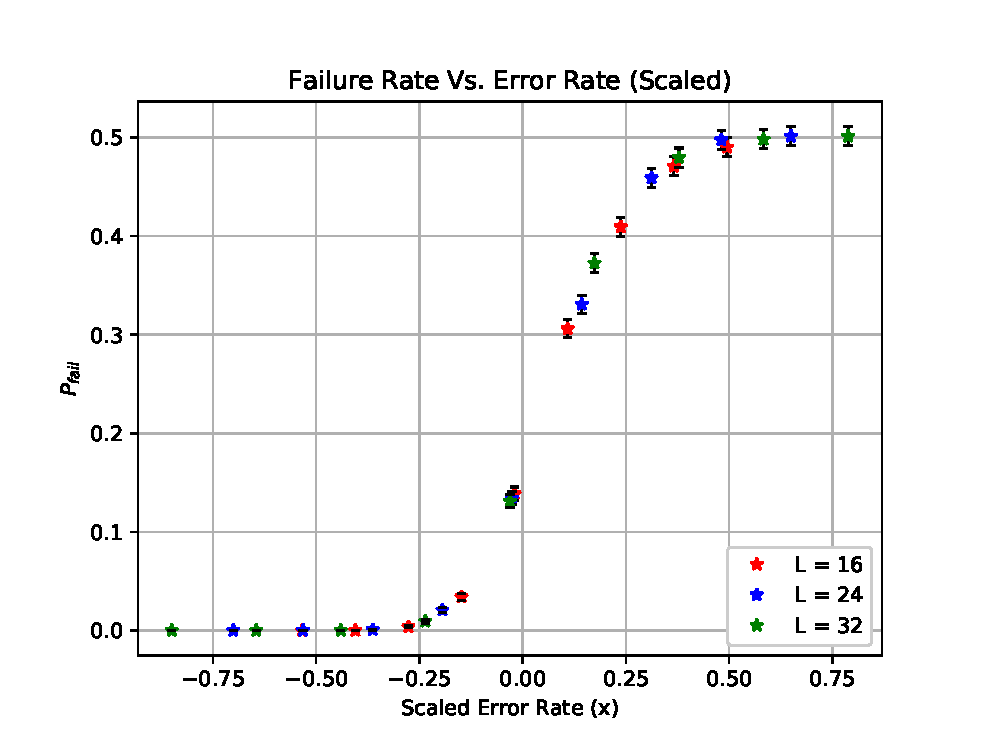
\includegraphics[width = \textwidth]{figs/scaled.eps}
			\caption{A plot of the rescaled data $x$ vs $P_{fail}$. $v_c = 1.49$, $p_c = 0.103$}
			\label{fig:scaled}
	\end{minipage}
	
	\end{figure}
	Data provided by figure \ref{fig:unscaled} determined $p_{c0}$ to be $0.103\pm 5$ ($10.3\pm 5 \%$ error), through the use of hyperbolic tangent trendlines.
\section{Correlated Errors}
\begin{figure}[htpb]
	\centering
	\includegraphics[width = 0.7\textwidth]{figs/30x30.png}
	\caption{A L=30 code with 5000 samples, showing both the effect of the number of error chains, and the length of those error chains on the success rate of the code.}
	\label{fig:3dplots}
\end{figure}
It can be seen in figure \ref{fig:3dplots} that the success rate of the code is dependant upon both the number of anyons and the chain length. It is also apparent that degree of correlation of errors has a distinct effect on the success rate, as these plots are not symmetric over the line of constant error rate. Figure \ref{fig:IncreasingCorr} shows that when the total number of errors is kept constant and the degree of correlation is increased, the failure rate of the code increases. 
\begin{figure}[htpb]
	\centering
	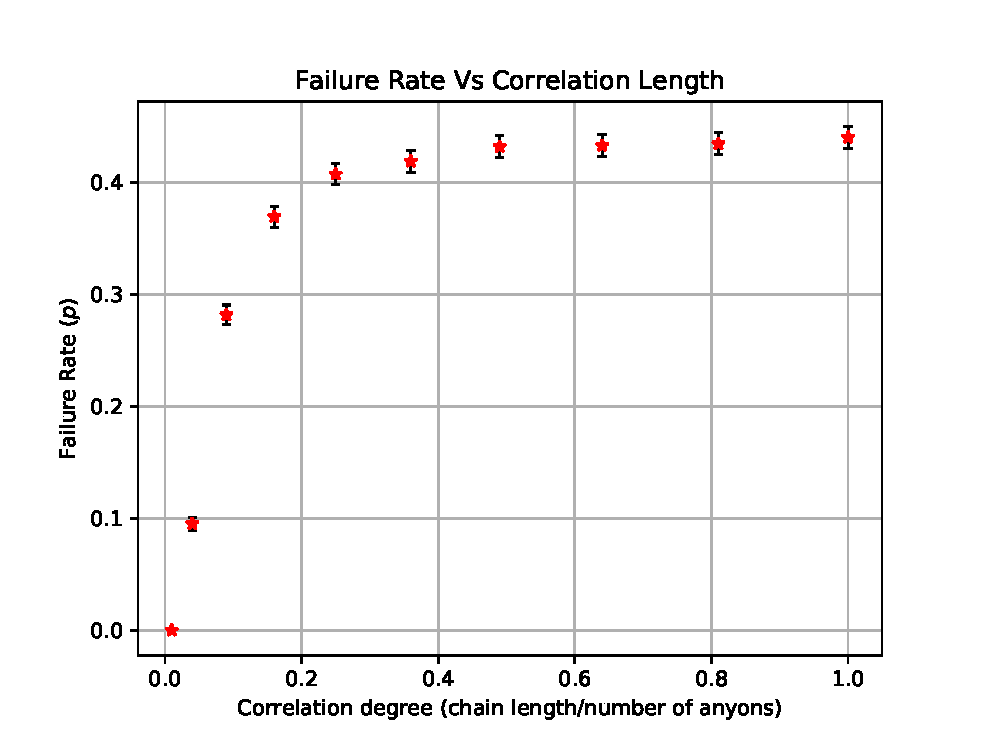
\includegraphics[scale = 0.7]{figs/pvscorr.eps}
	\caption{A 60x60 grid, with a constant number of error sites (11.1$\%$ of sites had error). This means that as the correlation length of the chains was increased, the number of chains was decreased, to keep the total number of affected sites constant. It can be seen that as the correlation length of the anyon gets longer, their failure rate increases; even with the total number of affected sites remaining constant. }
	\label{fig:IncreasingCorr}

\end{figure}


\section{Improved decoder}
initially we run the decoder with a variance of 1, and sweep the centre of th gaussian ($\overline{x}$) to determine if correcting for error correlations has any effect on the failure rate of the code. 
\begin{figure}[htpb]
	\includegraphics{figs/var1xbarvsfailure}
	\caption{this plot shows how the code implemented allows the code to match the failure rate of the origional code, even though it isnt least weight. this means that my code should work, with better parameters.}
	\label{fig:xbarplot1}
\end{figure}
Given that the adjusted code doesnt fail more than the origional code, up until a value close to the expected walk length predicted by all three methods, we shall use the a point near these predicted walk lengths to varying the next parameter in out gaussian, to attempt to improve the failure rate. 

Next we vary the variance ($\sigma^2$) of the gaussian correction, in an attempt to find an optimal value, so that we can again sweep over $\overline{x}$ to determine which distribution is the best to apply to reduce the failure rate further. 

\begin{figure}[htpb]
	\includegraphics{figs/improvementl300000L40True_3398b43b399345d183a59bfda7727a61.pdf}
	\caption{This plot shows how the variance has a very interesting curve, for what variances can be optimal. This likely has effects/interactions from the other walks in locality. An optimal variance was found at $\sigma^2$ = 10.75. Variance was stepped in sizes of 0.5.}
	\label{fig:varplot}
\end{figure}
Figure \ref{fig:varplot} shows clearly how for certain variances, the improved decoder with gaussian walk length correction beats the least weight perfect matching algorithm used for uncorrelated errors. We will now used this value of 10.75 to perform a higher another run of sweeping $\overline{x}$ to determine which distribution/expected length's distribution should be most optimal. 




The first naive simulation we run is with a gaussian correction, to reduce the adjusted weight smaller near the RMS distance of the walk. Once we have good data from this, we shall then compare to the other distance methods to determine which is the best expected distance/distribution to use to design the optimal decoder. 

Using an expected walk length of 5.016, we vary the the variance of the 



\section{Correction schemes}

Two correction schemes were used to attempt to lower the failre rate. one method was a concatenation of the least weight linear relationship with a gaussian drop in distance close to the expected walk length. 
A THIRD CORRECTION SCHEME COULD BE TO CONCATENATE THE GAMMA FUNCTIONS WITH THE LINEAR SCALING SAME AS FOR THE RAW GAMMA FUNCTION


the other method was to determine the actual distribution of walk lengths, and reduce the distance of syndrome measurements accordingly.

\begin{figure}[htpb]
	\centering
	\includegraphics[width= 0.5\textwidth]{figs/gamma_corrections.png}
	\caption{this is how the distances were reduces accoring to the distributions}
	\label{fig:gamma}
\end{figure}
as canbe seen in \ref{fig:gamma} the distributions were adjusted to a peak height of unity, and were then inverted, to reduce the distances near the expected walk length. The distribution needed to be extended beyond the point of N as neighbouring walks can have a larger distance. The max distance should be sqrt(2*L*L)/2 +1 as this is the largest possible disagonal distance on the torus. 
\begin{itemize}
	\item generate x random walks 
	\item calculate gamma function parameters from this distribution
	\item calulate gaussian
	\item flip and create new weighting function
	\item apply for y code simulations and determine new failure rates
\end{itemize}

\section{Performance of Gaussian Correction}

\begin{figure}[htpb]
\centering
	\includegraphics[width = 0.7\textwidth]{figs/A4N32l40000.pdf}
\caption{This figure shows the performance of the gaussian correction for $\sigma^2$ and $\overline{w}$ when 4 anyons are present with N=32 on a L=40 code.}
\label{fig:A4rough}
\end{figure}

Figure \ref{fig:A4rough} shows a similar trend to other anyon densities. However, even with 40,000 loops per point, the error rate is so low ($\overline{p} = 0.00314\pm 0.00002$) that resolving dependence on variables is difficult, as it becomes computationally difficult to reduce relative errors at this rate. For this reason higher numbers of anyons are primarily studied to decrease computation time.

\begin{figure}
\centering
\includegraphics[width = 0.7\textwidth]{figs/variancevslocation_combined.pdf}
\caption{A large range scan of N=32 A=15 for $\sigma^2$ and $\overline{w}$}
\label{fig:A15rough}
\end{figure}
The variance was studied to very large values ($\sigma^2 = 40$) and a trend seems to form. As the variance is increased, the `best' $\overline{w}$ also walks up.




\section{Comparison of expected walk length methods}

\begin{figure}[htpb]
	\centering
	\includegraphics[width = 0.7\textwidth]{figs/comparison_of_methods}
	\caption{This trend clearly shows that the gaussian benefits from being centered at the expected walk length calculated from the pythagorean method of walk lengths. }
	\label{fig:methodcomparison}
\end{figure}
Figure \ref{fig:methodcomparison} is not conclusive in determining what is the optimal walk length to choose, however it does show that for the parameters used, the pythagorean distance gives the best success rate. All methods are more effective than the classical code, but pythag is best. \\
Obviously the next step is to run a higher accuracy scan over the 5.016 value, to determine if this is an accurate minimum, or just a coincidence. There is reason to believe that one of the three methods will be correlated to the best value for the mean; and that the best value, will be modulated from this calculation dependant upon the size of the code, and the anyon density, and the chain length. these `neighbour interactions' will likely dictate what the optimal parameters will be. This means that a practical implementation of the improved Toric code may require walking the parameters of the correction, until a global minimum of failure rate is found.  A good guess for the centre of the gaussian correction has however, been shown to any of the three expected walk length calculations; as all choices beat the classical code; for the current parameters. 

In the case of the gaussian, the centre of it may not even need to correspond exactly to one of the expected walk length calculations, as the gaussian is only approximating the actual walk length distribution of random walks. In the case where we correct using the actual distributions of random walks; we should see that it beats the gaussian for every parameter of the gaussian. 

The gamma functions however, may also need some degree of tuning to account for the `neighbour interactions'. 

%%%%% Conclusion
\chapter{Conclusion}

	There are several short term goals of the project now that uncorrelated errors can be efficiently simulated. 
	
	Randomized benchmarking is a method for characterizing the failure rate of imperfect quantum gates. While this is a well established area of research for many application of quantum gates, randomized benchmarking has never before been applied to the Toric Code. A local check code like the Toric Code is known to be robust against localized errors, so investigating this behaviour with randomized benchmarking is an useful area of research. Developing an implementation of randomized benchmarking for the Toric code, and investigating the behaviour of a local check code with faulty gates is an important future goal of the project.
	
	Information about correlation distances can be garnered from syndrome measurements. Optimizing the decoder performance using information gained from syndrome measurements about correlated error models should increase the success rate of the code. Improving the success rates of ECCs is much sought after, and is a priority of the project moving forward. 
	
	\section{Future work}
	
	Future work may include creating a bias for walks to travel in one direction. This would be akin to creating markov chain montecarlo method.
	
	 Other possible work could be having walks avoid each other? 
\bibliography{bib}
\appendix

%%%%% Projectors
\chapter{Appendix}
\section{Gamma functions}
a gamma distribution can be described by the equation: 
\begin{equation}
	f(x;\alpha,\beta)  = \frac{\beta^\alpha x^{\alpha-1} e^{-\beta x}}{\Gamma (\alpha)}
\end{equation}
where $\alpha$ is known as the shape parameter, and $\beta$ is known as the inverse scale parameter($\beta = 1/\theta$ where $\theta$ is the scale parameter)). $\Gamma(x)$ is described by;
\begin{align}
	\Gamma(n) &= (n-1)! \hspace{1cm} n\in \mathds{Z} \\
	&= \int_{0}^{\infty}x^{n-1} e^{-x} dx\hspace{1cm}   n\in \mathds{C}
\end{align}
taking the derivative of the gamma distribution we get:
\begin{align}
	f' & = \frac{d}{dx}\left(\beta^\alpha e^{-\beta x}x^{\alpha-1} \right) \\
	& =\beta^\alpha \left( x^{\alpha -1} \left(\frac{d}{dx}\left( e^{-\beta x} \right) \right) + e^{-\beta x }\left( \frac{d}{dx}\left( x^{\alpha -1} \right) \right) \right)\\
	& = \beta^\alpha \left( 	(\alpha -1 ) e^{-\beta x} x^{\alpha -2} + -\beta x^{\alpha -1}e^{-\beta x}    	\right) \\
	%& = 
\end{align}
equating to zero to find a maximum we get;
\begin{align}
	0 &= \beta^\alpha \left( 	(\alpha -1 ) e^{-\beta x} x^{\alpha -2} + -\beta x^{\alpha -1}e^{-\beta x}   \right) \\
	&=  (\alpha -1 ) e^{-\beta x} x^{\alpha -2} + -\beta x^{\alpha -1}e^{-\beta x} \\
	&=  (\alpha -1 ) x^{\alpha -2} + -\beta x^{\alpha -1} \\
	&= \frac{(\alpha -1 )x^{\alpha-1}}{x} - \beta x^{\alpha -1} \\
	&= \frac{\alpha  -1}{x} - \beta \\
	x & = \frac{\alpha -1}{\beta}
\end{align}


So a critical point (the maximum) occurs at $(\alpha -1)/\beta$ which corresponds to a maximum of;
\begin{align}
f\left( \frac{\alpha-1}{\beta};\alpha,\beta \right) & = \frac{\beta^\alpha \left( \frac{\alpha-1}{\beta}\right)^{\alpha -1} e^{-\beta \frac{\alpha-1}{\beta}}}{\Gamma(\alpha)}\\
\end{align}

For the project, gamma functions were fit to the distributions displacements by different metrics, for walks of a certain length using scipy.stats.gamma. Using this package, the form of the maximum after fit, is;

Where $loc$ is the offset of the centre of the distribution.
Scipy.stats.gamma also gives us the fit parameters in the form $[\alpha, loc, \theta ]$ or $[shape, location, scale]$ so theta must also me converted;
\begin{figure}

\end{figure}
\section{Manhattan Distance}
	The Manhattan distance is a way to describe the distance between two points in a reference frame, say (x1,y1) and (x2,y2), where the distance is defined not as the Pythagorean distance of; 
	$$D = \sqrt{(x1-x2)^2 + (y1-y2)^2}$$ 
	but as; 
	$$M = |x1-x2|+|y1-y2|$$ 


\section{Maths}
		\subsection{Definitions}
		\label{app:pauli}
		Pauli Matrices
		\[
		X = 
		\begin{bmatrix}
		0 & 1 \\
		1 & 0
		\end{bmatrix}
		, Y = 
		\begin{bmatrix}
		0  & -i \\
		i & 0
		\end{bmatrix}
		, Z = 
		\begin{bmatrix}
		1  & 0 \\
		0 & -1
		\end{bmatrix}
		, I = 
		\begin{bmatrix}
		1  & 0 \\
		0 & 1
		\end{bmatrix}
		\label{fig:pauli}
		\]
\subsection{Hadamard Gate}
\label{app:hadamard}
		The Hadamard gate can be used to convert a $\ket{0}$ into $ \frac{1}{\sqrt{2}}(\ket{0} +\ket{1})$ and $\ket{1}$ into $ \frac{1}{\sqrt{2}}(\ket{0} -\ket{1})$.
		It is represented by the transformation matrix:
		\[ H = 
				\frac{1}{\sqrt{2}}\begin{bmatrix}
				1  & 1 \\
				1 & -1
				\end{bmatrix}
				\]
		This transformation allows for concatenated error correcting codes to deal with X and Z errors using the same procedure. 
		\subsection{Homology Classes}
		\label{app:cycles}

		A cycle is a loop. On a torus a homologically nontrivial cycle corresponds to a horizontal or vertical chain extending over the periodic boundary conditions which forms a noncontractibel loop. Any chain homologically equivalent to these chains is also homologically nontrivial. These cycles do not form the boundary of any surface. A trivial cycle is equivalent to any cycle which forms the boundary of a surface. 
		
		A single non-contractible loop cannot be formed from stabilizers; only pairs of loops which form the boundary of a region one dimension higher than the boundary chain itself. Thus, only trivial homologies can be formed from stabilizer measurements. 
		\begin{figure}
		\centering
		\includegraphics[width = 0.4\textwidth]{figs/errors.eps}
		\caption{This figure shows the 4 nontrivial cycles on the torus. There are conjugate directions for each chain of X and Z operators. Two of the cycles exist on the grid, and 2 exist on the co-grid.}
		\label{fig:errors}
		\end{figure}
		A linear combination of 2 rings around the torus forms the boundary of a 2D surface (an empty cylinder) which is 1D higher than the cycles forming the boundary; which means the homology is trivial.
		
		On the toric code, a homologically nontrivial loop does not commute with the hamiltonian. Trivial loops, such as those created by strings of stabilizers, commmute with the hamiltonian. 
		
\section{Code}
	This section contains small logically important snippets of the code are included here. 800 lines of core code was developed, along with supporting code for data processing, interfacing with code borrowed from Nickerson \cite{Nickerson2014}, and graphical displays.	
	\\\\
	Full code can be found at \url{https://github.com/gorff/Toric-Code-Correlated-Error-Decoder}.
		
		\begin{lstlisting}[language=Python, caption=Applying Uncorrelated Errors, label = code:applyerrors]
def ApplyUncorrelatedErrors( ErrorNum,array,type,L,CorrLen):
	#run across every element in the array
	for i in range(len(array[:,0,0])):
	   for j in range(2):
	       for k in range(len(array[0,0,:])):
	           if random.random() >1-ErrorRate: #rand chance of bitflip
	               array[i,j,k] = -1*array[i,j,k] #apply bitflip if true
	return(array)
		\end{lstlisting}


 
\backmatter

%%%%% Bibliography, in BibTeX format (the .bib file)
\bibliography{thesis}

\end{document}
